\shorthandoff{"}
\chapter{Person-Environment Fit}
\label{ch:personEnvironmentFit}

\section{Einführung}
\label{ch:personEnvironmentFit:einfuehrung}
%Edwards 2008
Der \acf{PEFit} \cite[S. 428]{dawis:2002} ist ein Konzept, welches häufig im Kontext der Berufs- und Organisationspsychologie angewendet wird \cite[S. 2]{guan:2021}. In manchen Publikationen findet sich die Theorie auch unter ähnlichen Bezeichnungen mit derselben Bedeutung wie Match \cite[S. 2]{player:2017}, Korrespondenz \cite[S. 1]{eggerth:2008} oder Kongruenz \cite[S. 1]{muchinsky:1987}. Es enthält stets drei zentrale Größen: Person, Umgebung (Environment) und Ergebnis (Outcome) \cite[S. 2f.]{livingstone:1997}.

\textcite[S. 5]{edwards:2007} stellten fest, dass die Literatur unter der Person ein menschliches Individuum versteht. Umgebung und Ergebnis interpretierten verschiedene Publikation ihren Beobachtungen zu Folge dagegen als breite Terminologien. Diese wurden je nach Forschungsdomäne genauer spezifiziert. Beispiele für Ergebnisse sind Zufriedenheit \cite[S. 1]{lashani:2021}, Wechselbereitschaft \cite[S. 1]{amarneh:2021}, Kreativität \cite[S. 1]{duan:2019}, Leistung \cite[S. 7f.]{elfenbein:2007} und  Berufswahl \cite[S. 1]{cable:1996}. Als Umgebung untersuchten verschiedene Publikationen unter anderem Unternehmen \cite[S. 1]{kristof:1996}, Gruppen \cite[S. 1]{werbel:2001} und Arbeitsplätze \cite[S. 1]{lu:2014}. 

Der \ac{PEFit} gibt dabei an, zu welchem Grad sich die untersuchten Werte von Person und Umgebung auf einem Niveau befinden \cite[S. 3]{chatman:1989}. Dabei wird der Fit nicht als Zustand, sondern als wechselseitiger Prozess betrachtet. In diesem interagieren Person und Umgebung miteinander und verändern sich dabei gegenseitig \cite[S. 21f.]{roberts:2006}. Diese Modifikationen können die Kongruenz sowohl verbessern als auch verschlechtern \cite[S. 4]{caplan:1987}. Aus diesem Grund wurden in der Literatur auch Maßnahmen erforscht, welche den \ac{PEFit} gezielt optimieren sollen \cite[S. 16]{cable:2001}.

Die Wissenschaft geht davon aus, dass ein Ergebnis stets vom Zusammenspiel von Person und Umgebung abhängig ist und nicht durch eine der beiden Größen alleine bestimmt wird \cite[S. 1]{muchinsky:1987}. Wie in Abbildung \ref{fig:personEnvironmentFit:einfuehrung:abb1} verdeutlicht, ist der Fit somit selbst kein Ergebnis, sondern eine unabhängige Variable, welche zur Bestimmung eines untersuchten Resultates herangezogen wird \cite[S. 4f.]{edwards:1991}.

\begin{figure}[h]
	\centering
	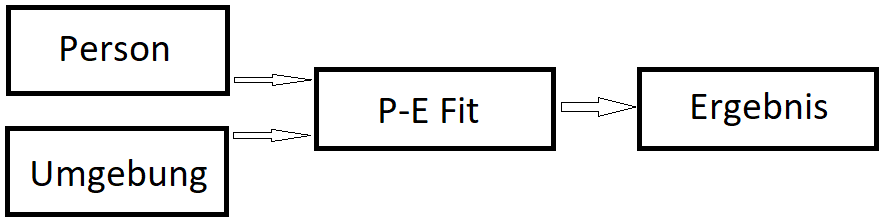
\includegraphics[width=1\textwidth]{gfx/P-E Fit.png}
	\caption{Zusammenwirken von Person, Umgebung, P-E Fit und Ergebnis / Nochmal schön machen und kennzeichnen, dass die P-E-Beziehung wechselseitig ist}
	\label{fig:personEnvironmentFit:einfuehrung:abb1}
\end{figure}
\newpage
\textcite[S. 6f.]{edwards:2007} unterschieden drei Ebenen, auf welchen ein Fit bestimmbar ist. Die Oberste bezeichneten sie als globale Ebene. Hier werden Person und Umgebung meist als Ganzes ohne weitere Untergliederungen miteinander vergleichen. Von der Domänen-Ebene sprachen \textcite[S. 7f.]{edwards:2007}, wenn eine Einteilung in mehrere sehr breite Bereiche vorgenommen wird, welche stellvertretend für Person bzw. Umgebung miteinander vergleichen werden. Domänen können den Autoren zu Folge beispielsweise Werte, Persönlichkeit oder Ziele sein. Findet die Untersuchung ausschließlich innerhalb einer Domäne statt, bezeichneten \textcite[S. 7f.]{edwards:2007} dies als Facetten-Ebene. Als Beispiel nannten die Wissenschaftler die Bestimmung eines \acp{PEFit} hinsichtlich demographischer Ähnlichkeit anhand von Dimensionen wie Alter und Bildung.

Wie die Kongruenz von Person und Umgebung berechnet wird, ist von der konkreten Art des Fits abhängig. \textcite[S. 1]{muchinsky:1987} unterschieden dabei zwischen ergänzendem (supplementary) und komplementären (complementary) Fit.

\section{Ergänzender und komplementärer Fit}
\label{ch:personEnvironmentFit:supplementaryUndComplementary}
Ein ergänzender Fit entsteht, wenn Person und Umgebung gleiche Werte und Interessen aufweisen \cite[S. 2f.]{muchinsky:1987}. Diese Art von Kongruenz ist laut \textcite[S. 1ff.]{schneider:1987} ein entscheidender Faktor, von welchen Unternehmen sich potentielle Arbeitnehmer angezogen fühlen und welche Bewerber von Betrieben eingestellt werden. \textcite[S. 4, Z. 25f.]{popovich:1982} zu Folge kann der Beitritt einer Person zu einem Unternehmen sogar als ein "sehr konkreter, öffentlicher Ausdruck der Werte"\footnote{"a very concrete, public expression of values" - \textcite[S. 4, Z. 25f.]{popovich:1982}} eines Individuums interpretiert werden. In diesem Kontext führten \textcite[S. 7]{devendorf:2008} eine Untersuchung bezüglich der Arbeitgeberattraktivität von Bekleidungsgeschäften durch. Hierbei stellten sie bestätigend fest, dass Frauen im Hochschulalter eine stärkere Anziehung zu denjenigen Betrieben als potentiellem Arbeitgebern verspürten, bei deren Mitarbeitern sie eine hohe Ähnlichkeit zu sich selbst wahrnahmen.

Verschiedene Autoren diskutierten die Ergebnisse des ergänzenden Fits in der Literatur kontrovers. \textcite[S. 6]{schneider:1987} stellte fest, dass Angestellte mit einer geringen Werte-Übereinstimmung eher dazu tendieren, ihr Unternehmen zu verlassen. So entsteht dem Autor zu Folge im Betrieb langfristig eine hohe Homogenität innerhalb der Belegschaft. Diese äußert sich einerseits in positiven Ergebnissen wie einer ausgeprägten Arbeitszufriedenheit, geringer Bereitschaft den Arbeitgeber zu wechseln und starker Identifikation mit dem Unternehmen \cite[S. 25ff.]{kristof:1996}\cite[S. 5]{su:2015}. Die mangelnde Diversität führt aber anderseits auch zu negativen Folgen, wie einer geringeren Bereitschaft für Veränderungen \cite[S. 10]{schneider:1987} und verminderter Kreativität und Innovation im Unternehmen \cite[S. 7]{chatman:1998}.

Wenn sich Person und Umgebung nicht ähneln, sondern gegenseitig vervollständigen, sprachen \textcite[S. 4]{muchinsky:1987} vom komplementären Fit. Dabei gleichen Person und Umgebung den Autoren zu Folge Schwächen des anderen durch eigene Stärken aus.

Die komplementäre Kongruenz wird, wie in Abbildung \ref{fig:personEnvironmentFit:supplementaryUndComplementary:abb1} dargestellt, in zwei weitere Fits untergliedert. Bei dieser Betrachtungsweise haben Person und Umgebung je eine Angebots- und eine Nachfrageperspektive. Die Nachfrage der einen Partei wird dabei durch das Angebot der anderen erfüllt \cite[S. 2ff.]{caplan:1987}\cite[S. 2f.]{edwards:1991}\cite[S. 2]{copingAndAdaption:1974}.

\begin{figure}[h]
	\centering
	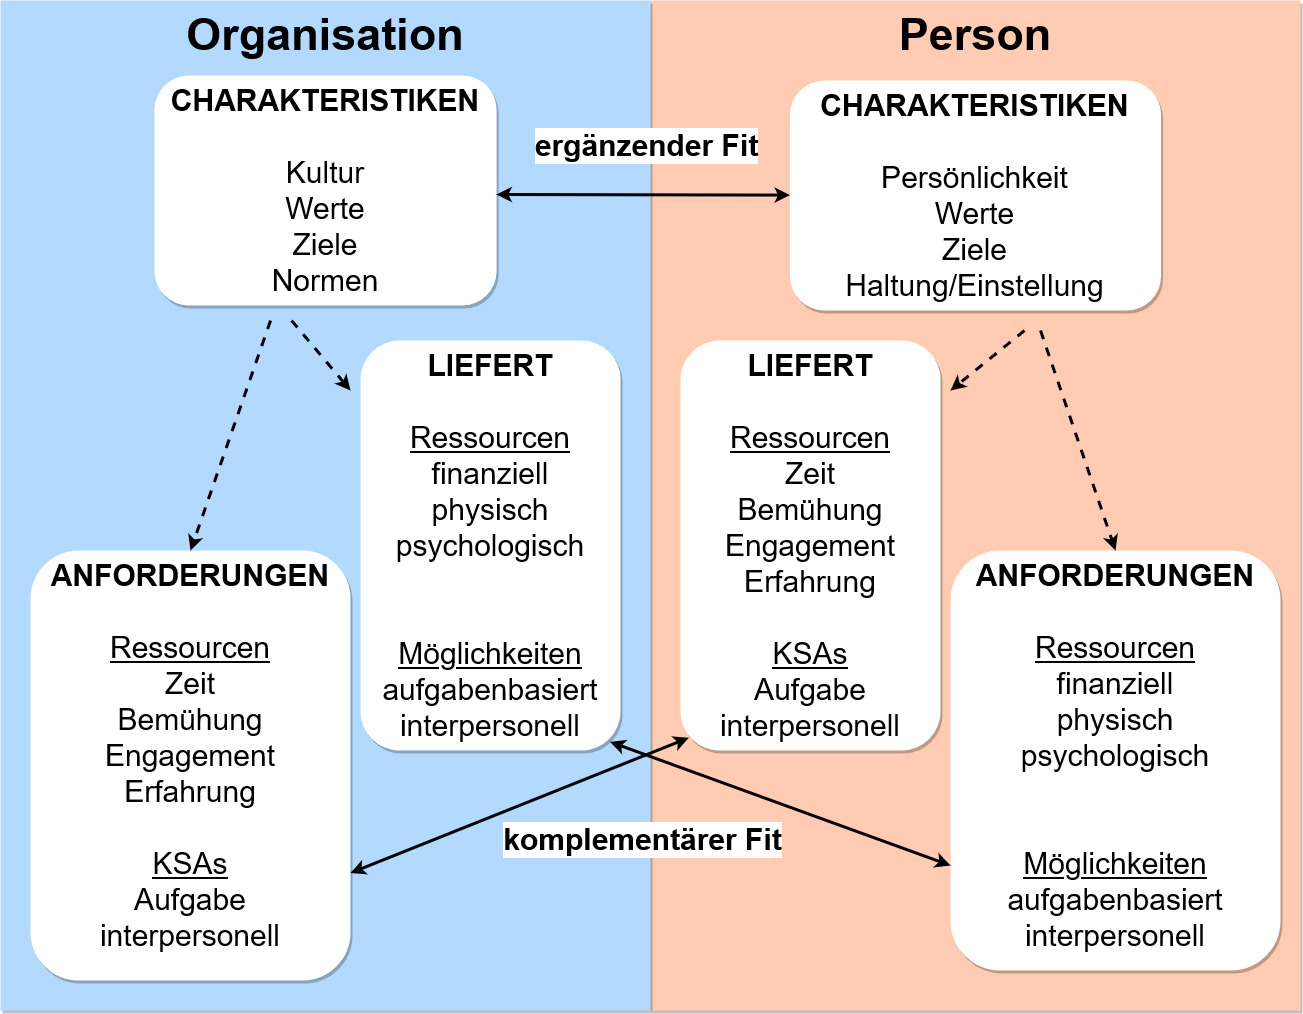
\includegraphics[width=1\textwidth]{gfx/supplementaryComplementaryFit.png}
	\caption{Ergänzender und komplementärer P-E-Fit \cite[S. 4]{kristof:1996}}
	\label{fig:personEnvironmentFit:supplementaryUndComplementary:abb1}
\end{figure}

Unter der Nachfrage der Umgebung werden die in Abbildung \ref{fig:personEnvironmentFit:supplementaryUndComplementary:abb1} dargestellten Anforderungen (Demands) an die Person zusammengefasst. Hierzu zählen beispielsweise Rollen- und Leistungserwartungen. Das entsprechende Angebot der Person sind ihre Fähigkeiten (Abilities). Diese umfassen unter anderem Fertigkeiten, Wissen, Bildung und Arbeitserfahrung. Gleichen sich Nachfrage der Umgebung und Angebot der Person gegenseitig aus, entsteht der Anforderungen-Fähigkeiten Fit (Demands-Abilities Fit). Dieser resultiert in einer hohen Leistung und Effizienz von Individuum und Umgebung \cite[S. 3f.]{edwards:1991}\cite[S. 5]{edwards:1996}\cite[S. 4f.]{edwards:2007}\cite[S. 6]{su:2015}.

Die Nachfrage der Person entspricht ihren psychologischen Bedürfnissen (Needs). Dazu zählen persönliche Präferenzen, Interessen, Motive und Ziele. Die entsprechenden Angebote (Supplies) der Umgebung umfassen Ressourcen und Belohnungen wie Gehalt und Mitbestimmungsrechte, welche die Bedürfnisse des Individuums befriedigen. Sind Nachfrage der Person und Angebote der Umgebung gleich stark ausgeprägt, wird dies in der Literatur als Bedürfnisse-Angebote Fit (Needs-Supplies Fit) bezeichnet. Dieser resultiert in einem hohen Wohlbefinden des Mitarbeiters, welches sich beispielsweise in Zufriedenheit und verminderter Wechselbereitschaft äußert \cite[S. 2]{edwards:2004}\cite[S. 2f.]{edwards:1996}\cite[S. 4]{edwards:2008}\cite[S. 4f.]{edwards:2007}\cite[S. 6]{su:2015}.

% und \textcite{wanous:1992}
% Charakteristiken auch beim komplementären Fit 
Laut \textcite[S. 9ff.]{workAdjustment:1964} führen unausgeglichene Nachfragen langfristig zu einem Wechsel des Arbeitsplatzes. Die Autoren betrachteten die aus unzureichend erfüllten Anforderungen des Unternehmens entstehende mangelnde Arbeitsleistung als Ursache für Kündigung oder Versetzung des Mitarbeiters seitens des Arbeitgebers. Die aus unzureichend erfüllten Bedürfnissen des Angestellten resultierende Unzufriedenheit bezeichneten die Wissenschaftler als einen Wechselgrund seitens des Mitarbeiters.
%"Wenn die Bedürfnisse jeder Entität von der anderen erfüllt werden und beide ähnliche grundlegende Eigenschaften teilen"\footnote{"when each entity’s needs are fulfilled by the other and they share similar fundamental characteristics" - \textcite[S. 6]{kristof:1996}}, ist laut \textcite[S. 6]{kristof:1996} ein optimaler Fit erreicht.

\textcite[S. 1ff.]{edwards:2004} charakterisierten ergänzende und komplementäre Kongruenz als unterschiedliche, parallele Strömungen innerhalb der \ac{PEFit}-Forschung. Doch sie stellten fest, dass beide Fits nicht vollkommen unabhängig voneinander sind. Die Ursache sahen sie in den inneren Werten von Person und Umgebung. Diese sind den Autoren zu Folge einerseits ausschlaggebend für den ergänzenden Fit, beeinflussen aber auch stark die Bedürfnisse der Person und die Angebote der Umgebung. Beispielsweise könnte sich ein Individuum mit ausgeprägten familiären Werten aufgrund des ergänzenden Fits stark zu Betrieben mit einer gemeinschaftlichen Unternehmenskultur angezogen fühlen. Gleichzeitig prägt die Person aufgrund ihrer inneren Werte im komplementären Fit das Bedürfnis nach familiären Reizen wie gemeinsamen Veranstaltungen aus. Da das Unternehmen dieselben Eigenschaften besitzt, wird es eher dazu tendieren, seinen Mitarbeitern die Teilnahme an derartige Ereignisse anzubieten.

Dass der Abgleich der Charakteristiken von Person und Umgebung sehr bedeutsam für Zufriedenheit und Produktivität sind, erkannten Psychologen bereits vor über einhundert Jahren \cite[S. 5ff.]{parsons:1909}. Die Wurzeln des \acp{PEFit} reichen zurück bis ins Jahr 1909 \cite[S. 1]{su:2015}.

\section{Historische Entwicklung}
\label{ch:personEnvironmentFit:historisches}
% Wie schreibt man hier "Männer" ohne dass es komisch ist?
Im ersten Jahrzehnt des 20. Jahrhunderts beschäftigten sich Wissenschaftler und Psychologen in zahlreichen Ländern der westlichen Welt intensiv mit dem Thema der Personalauswahl \cite[S. 1]{salgado:2001}. Ein Hauptanliegen der Forscher war es, individuelle Unterschiede zwischen den Menschen anzuerkennen und bei der Berufswahl zu berücksichtigen \cite[S. 2ff.]{stern:1900}. Deren Ansichten zu Folge würde die gesamte Gesellschaft effizienter arbeiten, wenn Menschen eine zu ihren wissenschaftlich ermittelten Fähigkeiten passende Tätigkeit aufnehmen würden \cite[S.2]{kevles:1968}\cite[S. 3]{parsons:1909}. Im Zuge dieser Entwicklungen konzipierte der Bostoner Professor Frank Parsons eine Vorgehensweise zur Berufsfindung für junge Männer, welche im Jahr 1909 vorgestellt wurde \cite[S. 1]{su:2015}. \textcite[S. 5ff.]{parsons:1909} erkannte schon zum damaligen Zeitpunkt, dass das Gleichgewicht von eigenen Fähigkeiten und Anforderungen des Berufsumfeldes eine wichtige Ursache für Effizienz, Produktqualität und Bezahlung waren. Aus diesem Grund empfahl er jungen Männern vor der Berufswahl zunächst ihre eigenen Fähigkeiten, die Anforderungen verschiedener Arbeitsplätze und die Beziehung zwischen beiden Seiten zu verstehen. Erst wenn sie diese Punkte unter Beaufsichtigung eines Berufsberaters und durch Verwendung verschiedener wissenschaftlicher Tests erfüllen, können sie sich dem Autor zu Folge für einen passenden Beruf entscheiden. Heute gilt Parsons aufgrund dieser Gedanken als "Gründungsvater der Berufsberatung"\footnote{"founding father of vocational guidance" - \textcite[S. 3, Z. 29]{porfeli:2009}} \cite[S. 3, Z. 29]{porfeli:2009} und als erster Vorläufer des \acp{PEFit} \cite[S. 2]{edwards:2008}.

Zum damaligen Zeitpunkt begegnete die Bevölkerung den neuartigen psychologischen Tests zunächst mit Skepsis \cite[S. 2]{kevles:1968}. Das änderte sich insbesondere im Jahr 1917 mit dem Eintritt der Vereinigten Staaten in den Ersten Weltkrieg. Das U.S. Militär stand vor der Herausforderung, innerhalb kürzester Zeit Millionen Männer in die verschiedenen spezialisierten Rollen des technisierten Krieges einzuordnen. Zu diesem Anlass setzten Wissenschaftler erstmals im großen Stil psychologische Tests zur Zuweisung von Personen zu passenden Militärpositionen ein \cite[S. 2ff.]{kevles:1968}. 

Nach dem Ersten Weltkrieg entstanden insbesondere in den 1930er-Jahren durch die Arbeiten der Wissenschaftler \textcite[S. 1ff]{lewin:1936} und \textcite[S. 1ff.]{murray:1938} weitere bedeutende Entwicklungen für die Entstehung des \acp{PEFit} \cite[S. 1]{edwards:1990}. \textcite[S. 11f.]{lewin:1936} stellte fest, dass das Verhalten eines Menschen nicht, wie bis dahin angenommen, nur durch das Individuum selbst, sondern durch das Zusammenspiel von Person und Umgebung zu erklären ist. Ähnlich zu diesen Erkenntnissen erarbeitete \textcite[S. 38ff.]{murray:1938} sein Need-Press-Modell. Der Wissenschaftler ging davon aus, dass jeder Mensch im Laufe seines Lebens verschiedene Bedürfnisse (Needs) unterschiedlich stark ausprägt. Diese treffen je nach Umgebung auf diverse Reize. Murray stellte fest, dass manche Reize mit bestimmten Bedürfnissen kompatibel sind. Trifft ein passendes Bedürfnis-Reiz-Paar aufeinander, entsteht Druck (Press). Personen interpretieren diesen subjektiv als schädliche oder nützliche Situation und zeigen dem Autor zu Folge eine entsprechende Reaktion. Dieses Zusammenspiel von Bedürfnissen einer Person und Reizen der Umgebung entspricht der späteren Vorstellung des Bedürfnisse-Angebote Fits \cite[S. 8]{edwards:2008}. 

Die Erkenntnisse von \textcite[S. 1ff]{lewin:1936} und \textcite[S. 1ff.]{murray:1938} gelten als wichtiger Grundstein für die Arbeiten verschiedener Forschungsgruppen rund um John R. P. French, Jr. \cite[S. 5]{caplan:1993}. Der Psychologe stellte im Jahr 1963 an der Universität in Michigan ein groß angelegtes Forschungsprogramm vor. Dieses machte es sich zum Ziel, die Auswirkungen des sozialen Umfeldes in Industrieunternehmen auf die Gesundheit der Mitarbeiter zu untersuchen. Zu diesem Zweck arbeiteten Experten verschiedener Fachrichtungen eng zusammen \cite[S. 1ff.]{french:1963}. Aus dieser Kollaboration entstanden wesentliche formale Definitionen des \acp{PEFit}, welche beispielsweise von \textcite[S. 1ff.]{copingAndAdaption:1974} öffentlich präsentiert wurden. In dieser Publikation unterschieden die Forscher, ausgehend ihren bis dahin erzielten Erkenntnissen, zwischen objektivem und subjektivem Fit \cite[S. 4f.]{caplan:1993}\cite[S. 1ff.]{french:1966}.

\section{Objektiver und subjektiver Person-Environment Fit}
\label{ch:personEnvironmentFit:subjektivObjektiv}
% Hierzu Quellen von Caplan und Harrison einfügen, sobald Bücher verfügbar
Wie in Abbildung \ref{fig:personEnvironmentFit:subjektivObjektiv:abb1} dargestellt, gingen \textcite[S. 1ff.]{copingAndAdaption:1974} davon aus, dass von Person und Umgebung je eine objektiv messbare und eine vom Individuum subjektiv wahrgenommene Version existieren.

\begin{figure}[h]
	\centering
	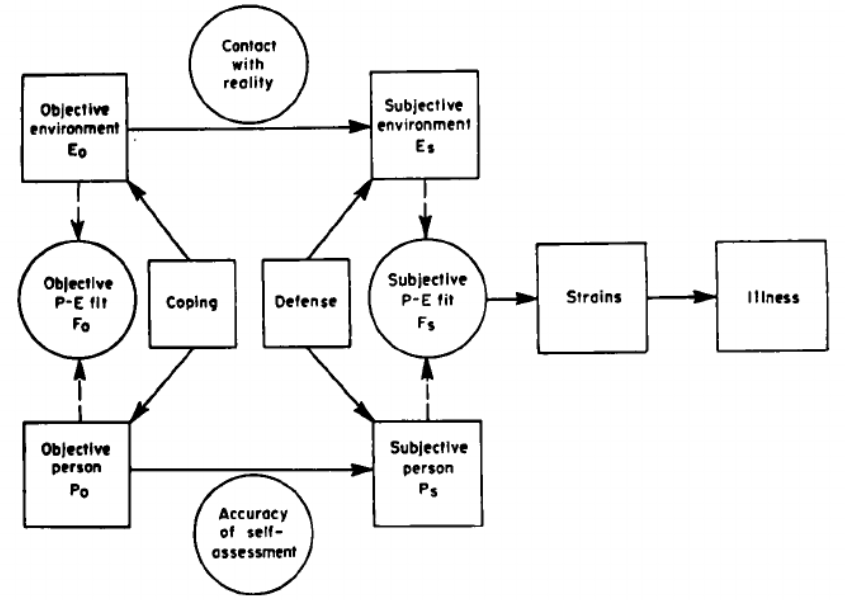
\includegraphics[width=1\textwidth]{gfx/subjektivObjektivPEFit.png}
	\caption{Objektiver und subjektiver P-E Fit \cite[S. 22]{edwards:2008}}
	\label{fig:personEnvironmentFit:subjektivObjektiv:abb1}
\end{figure}

% 4 Subjekte farbig markieren
Die Forscher betonten die Wichtigkeit, die vier in Abbildung \ref{fig:personEnvironmentFit:subjektivObjektiv:abb1} dargestellten Subjekte anhand vergleichbarer Dimensionen zu messen. Dies betrachteten sie als wichtige Grundlage, um über Ähnlichkeitsberechnungen aussagekräftige Werte für den objektiven und subjektiven \ac{PEFit} zu bestimmen \cite[S. 2f.]{copingAndAdaption:1974}.

% Eig french und Kahn 1962 S. 10ff.
Aus der Publikation von \textcite[S. 10ff.]{french:1962} schlossen \textcite[S. 15]{copingAndAdaption:1974}, dass Individuen anstreben, unerfüllte Motive zu verhindern. Um dies zu erreichen, existieren den Wissenschaftlern zu Folge zwei Strategien. Ändert eine Person ihre objektive Umgebung oder ihr objektiv ermitteltes Selbst zur Verbesserung des objektiven \acp{PEFit}, sprachen \textcite[S. 15f.]{copingAndAdaption:1974} von Bewältigung (Coping). Ändert das Individuum ihre subjektive Wahrnehmung von Umgebung oder sich selbst zur Optimierung des subjektiven \acp{PEFit}, bezeichneten sie die Strategie als Verteidigung (Defense).

Beispielsweise könnte sich ein Bachelor-Absolvent für eine Stelle interessieren, welche als Anforderung einen Master-Abschluss voraussetzt. Diese Unterschiede im objektiven \ac{PEFit} könnte die Person bewältigen, indem sie entweder den fehlenden Abschluss erwirbt oder das Unternehmen überzeugt, die Stellenanforderungen abzuändern. Dagegen könnte der Betrieb auch einen zukünftigen Mitarbeiter suchen, welcher über ein bestimmtes Kenntnisniveau in einer Programmiersprache verfügt. Schätzt ein potentieller Bewerber seine Fähigkeiten zunächst schlechter ein als gefordert, gerät der subjektive \ac{PEFit} ins Ungleichgewicht. Die Person kann sich hierbei verteidigen, indem sie die Wahrnehmung ihrer Kenntnisse nachträglich besser bewertet oder die Anforderungen der Stellenausschreibung abwertet.

\textcite[S. 4]{copingAndAdaption:1974} bemerkten außerdem, dass insbesondere der subjektive \ac{PEFit} bedeutsam für die Entstehung psychischer Belastungen ist. Auch Publikationen anderer Forscher bestätigten diese Einschätzung \cite[S. 3]{carless:2005}. Dementsprechend wurde die subjektive Wahrnehmung des \acp{PEFit} in der Literatur stärker fokussiert \cite[S. 8]{caplan:1987}\cite[S. 9]{caplan:1993}\cite[S. 16]{choi:2004}.

In einer auf den Erkenntnissen von \textcite[S. 1ff.]{copingAndAdaption:1974} aufbauenden Arbeit kam \textcite[S. 5ff.]{harrison:1978} sogar zu der Einschätzung, dass innerhalb des subjektiven \acp{PEFit} alleine die Bedürfnisse-Angebote Kongruenz Auswirkungen auf die mentale Gesundheit des Mitarbeiters hat. Ein Ungleichgewicht im Anforderungen-Fähigkeiten Fit führt dem Autor zu Folge dagegen nur dann zu psychischer Belastung, wenn diese der Erfüllung des Bedürfnisse-Angebote Fits schadet. Beispielsweise könnte sich ein Mitarbeiter von der Erfüllung einer Aufgabe zusätzliches Gehalt versprechen. Reichen dessen Fähigkeiten jedoch nicht aus, die Anforderungen zu erfüllen, könnte dessen Stressgefühl zunehmen. Der Grund für dessen psychische Belastung ist laut \textcite[S. 13]{harrison:1978} jedoch nicht das unterschiedliche Niveau von Fähigkeiten und Anforderungen als solches. Die Ursache für den Stress ist dem Autor zu Folge die nicht erreichte Gehaltsauszahlung, welche sich der Mitarbeiter wünschte. Somit löste das Ungleichgewicht im Anforderungen-Fähigkeiten Fit nur Stress aus, da die daraus resultierende Nichterfüllung der Aufgabe den Bedürfnisse-Angebote Fit ins Ungleichgewicht brachte.
% eine leistungsabhängige Gehalts-Auszahlung. Möchte ein Mitarbeiter die Bezahlung erhalten (Bedürfnis), welche vom Arbeitgeber in Aussicht gestellt wird (Angebot), hat aber nicht ausreichende Fähigkeiten, um die dafür notwendigen Anforderungen zu erfüllen, führt dies zu Unzufriedenheit.

Auch \textcite[S. 1ff.]{lazarus:1978} stellen fest, dass zu hohe Anforderungen nur dann Stress bei einem Individuum auslösen, wenn dieses durch die Nichterfüllung negative Konsequenzen befürchtete. Dabei kann es sich den Autoren zu Folge entweder um schädliche Folgen für die Gesundheit oder die Verletzung innerer Werte und Ziele handeln.

Ungleichgewichte im \ac{PEFit} werden häufig auch als Misfits bezeichnet \cite[S. 2]{edwards:2004}, \cite[S. 4]{kristof:1996}. Mögliche Auswirkungen von P-E Misfits wurden in der Literatur in verschiedenen Arbeiten diskutiert.

\section{Auswirkungen von P-E Misfits}
\label{ch:personEnvironmentFit:auswirkungenErhoehterAngebote}
% Auch \cite[S. 21f.]{edwards:2008} äußert sich zu Kurven und nennt Beispiele
% Quellen: Mechanisms of Job Stres and Strain; harrsion:1978; harrsion:1985; caplan iwo
% das hier ist eigentlich von Caplan 1980 oder french rodergs and cobb (laut Mechanisms of Job Stress and Strain)
\textcite{mechanismsOfJobStressAndStrain:1982} stellten fest, dass ein Bedürfnisse-Angebote Misfit in unterschiedlichen Konsequenzen resultieren kann. Diese sind in Abbildung \ref{fig:personEnvironmentFit:auswirkungenErhoehterAngebote:abb1} dargestellt.

% Bild auch in Coping und Adaption? Nein.
\begin{figure}[h]
	\centering
	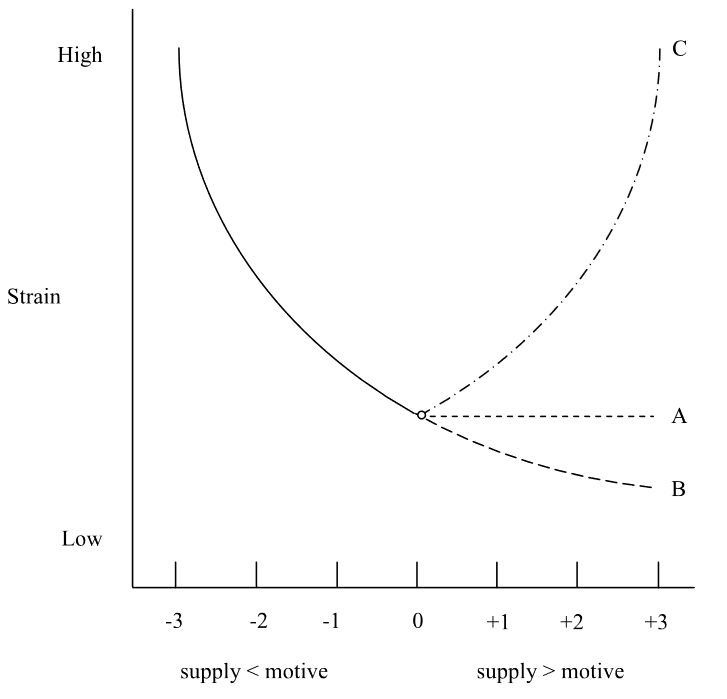
\includegraphics[width=0.75\textwidth]{gfx/ueberschuss_supply_motive.png}
	\caption{Auswirkungen eines Bedürfnisse-Angebote Misfits \cite[S. 23]{edwards:2008}\\(Bearbeitet von \myName)}
	\label{fig:personEnvironmentFit:auswirkungenErhoehterAngebote:abb1}
\end{figure}

An der durchgezogenen Linie auf der linken Hälfte von Abbildung \ref{fig:personEnvironmentFit:auswirkungenErhoehterAngebote:abb1} ist zu erkennen, dass je weniger die Bedürfnisse einer Person erfüllt werden, die mentale Belastung (Strain) des Individuums stärker zunimmt \cite[S. 30]{mechanismsOfJobStressAndStrain:1982}. Der Verlauf dieser Kurve kann über folgende algebraische Differenzberechnung bestimmt werden \cite[S. 2]{edwards:1993}:
\begin{equation}
	B = P - E
	\label{fig:personEnvironmentFit:auswirkungenErhoehterAngebote:formel1}
\end{equation}
In Gleichung \ref{fig:personEnvironmentFit:auswirkungenErhoehterAngebote:formel1} steht $B$ für die mentale Belastung des Mitarbeiters. $P$ stellt die von einer Person gewünschte Menge eines bestimmten Wertes dar. Die vom Mitarbeiter wahrgenommene erhaltene Menge des entsprechenden Wertes seitens der Umgebung wird über Parameter $E$ ausgedrückt \cite[S. 2]{edwards:1993}.

Übersteigen die Angebote der Umgebung die Bedürfnisse der Person, mündet dies in einer der drei gepunkteten Linien A, B oder C \cite[S. 29ff.]{mechanismsOfJobStressAndStrain:1982}.

% Hier noch eine zusätzliche Quelle?
Kurve A zeigt einen monotonen Verlauf der mentalen Belastung. Dieser entsteht, wenn eine Person die Übererfüllung eines Bedürfnisses entweder für einen späteren Zeitpunkt aufsparen oder in die Befriedigung verwandter Motive investieren kann. Dieser Sachverhalt ist beispielsweise erfüllt, wenn einer Person mehr Gehalt zusteht, als diese für die Zahlung ihrer Lebenskosten benötigt. Das überschüssige Geld könnte diese entweder für die Zahlung von Lebenshaltungskosten in den Folgemonaten aufsparen oder zusätzlich ihr mögliches Bedürfnis nach Luxusgütern befriedigen \cite[S. 30]{mechanismsOfJobStressAndStrain:1982}. Für die Berechnung von Kurve A kann ebenfalls Gleichung \ref{fig:personEnvironmentFit:auswirkungenErhoehterAngebote:formel1} verwendet werden \cite[S. 2]{edwards:1993}.

Linie B hat den Verlauf einer quadratischen Funktion und tritt ein, wenn die Übererfüllung eines Bedürfnisses entweder die Befriedigung dieses oder eines verwandten Motivs hemmt \cite[S. 5]{caplan:1987}. \textcite[S. 12]{harrison:1978} nannte hierfür das Bedürfnis einer Person nach sozialem Austausch als Beispiel, welches bei Übererfüllung das Verlangen nach Privatsphäre verletzt. Der Verlauf von Kurve B kann über die in Gleichung \ref{fig:personEnvironmentFit:auswirkungenErhoehterAngebote:formel2} dargestellte absolute Differenz bestimmt werden \cite[S. 2]{edwards:1993}.
\begin{equation}
	B = |P - E|
	\label{fig:personEnvironmentFit:auswirkungenErhoehterAngebote:formel2}
\end{equation}
Alternativ bietet sich die Verwendung der quadrierten Differenz aus Gleichung \ref{fig:personEnvironmentFit:auswirkungenErhoehterAngebote:formel3} an \cite[S. 2]{edwards:1993}.
\begin{equation}
	B = (P - E)^2
	\label{fig:personEnvironmentFit:auswirkungenErhoehterAngebote:formel3}
\end{equation}
Kurve C stellt eine asymptotische Beziehung zur mentalen Belastung dar. Sie tritt ein, wenn weder die Bedingungen von Kurve A noch von Linie B zutreffen. Eine Übererfüllung des Bedürfnisses hat folglich weder positive noch negative Auswirkungen auf die Person \cite[S. 30]{mechanismsOfJobStressAndStrain:1982}. Ein Beispiel für eine solche Beziehung ist ein Überangebot an Parkplätzen beim Arbeitgeber. Da der Mitarbeiter nur ein Fahrzeug besitzt, kann dieser von zusätzlichen Angeboten keinen Gebrauch machen und diese auch nicht für einen späteren Zeitpunkt aufsparen. Die zusätzlichen Parkplätze schaden auch keinem anderen Bedürfnis des Mitarbeiters. Somit entstehen weder positive noch negative Auswirkungen auf dessen Wohlbefinden. Zur Bestimmung von Kurve C wird die Belastung gleich dem Wert null gesetzt. Dieses Vorgehen ist in Gleichung \ref{fig:personEnvironmentFit:auswirkungenErhoehterAngebote:formel4} dargestellt \cite[S. 2]{edwards:1993}.
\begin{equation}
	B = 0
	\label{fig:personEnvironmentFit:auswirkungenErhoehterAngebote:formel4}
\end{equation}
Verschiedene Autoren gehen davon aus, dass die Beziehungen aus Abbildung \ref{fig:personEnvironmentFit:auswirkungenErhoehterAngebote:abb1} auch für den Anforderungen-Fähigkeiten Fit zu erwarten sind. Wie in Kapitel \ref{ch:personEnvironmentFit:subjektivObjektiv} beschrieben gilt dies nur, wenn das Erfüllen der Anforderungen Auswirkungen auf die inneren Werte des Mitarbeiters hat \cite[S. 12f.]{harrison:1978}. Wie an der durchgezogenen Linie auf der linken Seite von Abbildung \ref{fig:personEnvironmentFit:auswirkungenErhoehterAngebote:abb1} zu erkennen, entsteht in jedem Fall psychische Belastung, wenn die Anforderungen der Umgebung die Kenntnisse des Mitarbeiters übersteigen \cite[S. 5]{schuler:1980}. Sind dagegen die Fähigkeiten des Angestellten stärker ausgeprägt als erforderlich, resultiert eine der Kurven A bis C. Linie A tritt ein, wenn der Mitarbeiter seine gewonnenen Freiräume nutzen kann, um verwandte Bedürfnisse zu erfüllen. Schaden die zu niedrigen Anforderungen einem Bedürfnis des Mitarbeiters, entsteht Kurve B. Haben die zu hohen Fähigkeiten des Angestellten weder positive noch negative Auswirkungen auf dessen Wohlbefinden, resultiert Linie C \cite[S. 22f.]{edwards:2008}.

Unterschiedliche Publikationen stellten fest, dass der Verlauf der Kurven nicht alleine von den Auswirkungen der Misfits auf die Motive des Mitarbeiters abhängig ist. Zusätzlich muss beachtet werden, als wie wichtig der Angestellte die betroffenen Bedürfnisse bewertet \cite[S. 9f.]{edwards:1996}. 

\section{Einbeziehung der Wichtigkeiten von Bedürfnissen}
\label{ch:personEnvironmentFit:wichtigkeiten}
Bereits  \textcite[S. 7]{copingAndAdaption:1974} empfahlen die Einbeziehung von Wichtigkeitswerten in die Berechnung des \acp{PEFit}. Auf welche Weise diese Werte einbezogen werden sollten, ließen die Autoren zum damaligen Zeitpunkt jedoch unbeantwortet \cite[S. 19]{edwards:2008}.

\textcite[S. 38]{harrison:1985} schlug später vor, den \ac{PEFit} für jede untersuchte Variable einzeln zu berechnen und mit einem subjektiven Wichtigkeitswert zu multiplizieren. Diese Einschätzung teilte auch \textcite[S. 18]{locke:1969}\cite[S. 8f.]{locke:1976}. Er gilt als einer der einflussreichsten Wissenschaftler auf dem Gebiet der Arbeitszufriedenheit \cite[S. 12]{edwards:2008}. Diese kann laut \textcite[S. 8]{locke:1969} nur entstehen, wenn Mitarbeiter das Gefühl haben, für sie als wichtig erachtete Werte durch ihre Tätigkeit zu erfüllen. Aus diesem Grund empfahl er zur Berechnung der Arbeitszufriedenheit eines Angestellten zwei Kennzahlen heranzuziehen: Die Differenz aus wahrgenommener und gewünschter Menge eines Wertes und die subjektive Wichtigkeit des Motivs \cite[S. 8]{locke:1976}. \textcite[S. 16]{locke:1969} betonte, dass je nach untersuchtem Wert unterschiedliche Berechnungen wie algebraische oder absolute Differenz angewendet werden können. Ein Beispiel für eine Subtraktion mit algebraischer Differenz ist in folgender Gleichung \ref{fig:personEnvironmentFit:wichtigkeiten:formel1} dargestellt \cite[S. 9]{edwards:1990}:
\begin{equation}
	Y = b * (P - E)
	\label{fig:personEnvironmentFit:wichtigkeiten:formel1}
\end{equation}
In Gleichung \ref{fig:personEnvironmentFit:wichtigkeiten:formel1} steht $Y$ für das untersuchte Ergebnis, wie beispielsweise die Arbeitszufriedenheit. $b$ stellt den subjektiven Wichtigkeitswert dar. Dieser wird mit der Differenz aus gewünschter Menge eines Wertes einer Person $P$ und wahrgenommener Menge des Wertes der Umgebung $E$ multipliziert \cite[S. 9f.]{edwards:1990}.

Derartige Multiplikationen mit einem Differenzwert haben zur Folge, dass die in Abbildung \ref{fig:personEnvironmentFit:auswirkungenErhoehterAngebote:abb1} dargestellten Kurven mit steigender Wichtigkeit steiler werden \cite[S. 9]{locke:1976}. Abbildung \ref{fig:personEnvironmentFit:wichtigkeiten:abb1} verdeutlicht entstehende Stauchungen durch Wichtigkeitswerte.

\begin{figure}[h]
	\centering
	
	\subfloat[Algebraische Differenz]{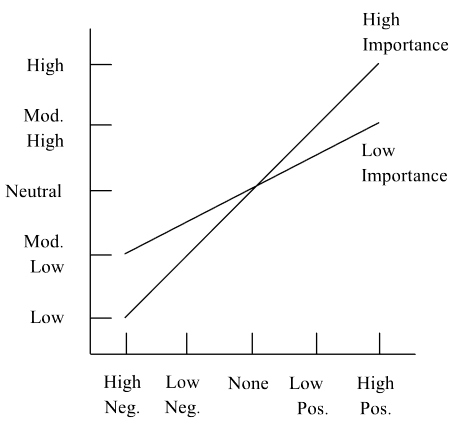
\includegraphics[width = 0.5\textwidth]{gfx/Locke-A.png}}
	\subfloat[Absolute Differenz]{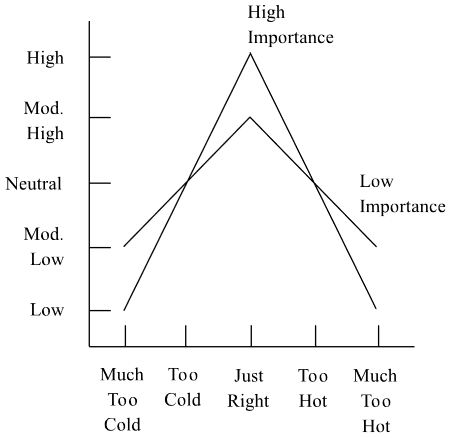
\includegraphics[width = 0.5\textwidth]{gfx/Locke-B.png}}
	
	\caption{Stauchung von Funktionsgraphen durch Wichtigkeitswerte \cite[S. 1305]{locke:1976}}
	%(Aus \cite[S. 13f.]{edwards:2008}, nach \cite[S. 1305]{locke:1976})
	\label{fig:personEnvironmentFit:wichtigkeiten:abb1}
\end{figure}

Im linken Teil (a) von Abbildung \ref{fig:personEnvironmentFit:wichtigkeiten:abb1} ist eine monotone Funktion basierend auf einer algebraischen Differenzberechnung dargestellt. Die rechte Seite der Grafik (b) zeigt den Verlauf einer Berechnung mit absoluter Differenz. In beiden Darstellungen ist zu erkennen, dass die Kurven bei geringer Wichtigkeit ausschließlich im mittleren Bereich von moderat niedrig bis moderat hoch verlaufen. Ist einem Individuum das jeweilige Bedürfnis dagegen sehr wichtig, füllt die Kurve den gesamten verfügbaren Bereich von niedrig bis hoch. Die Ausnutzung des größeren Gebiets führt zur Stauchung der Funktionsgraphen und damit zu einem stärkeren Ansteigen bzw. Absinken der Zufriedenheit des Individuums. 

\textcite[S. 51ff.]{edwards:1991}\cite[S. 9ff.]{edwards:1990}\cite[S. 2ff.]{edwards:1993}\cite[S. 2ff.]{edwards:1993b} kritisierte Berechnungen, wie in Gleichung \ref{fig:personEnvironmentFit:wichtigkeiten:formel1} dargestellt, in mehreren seiner Arbeiten. Dabei diskutierte er insbesondere die Multiplikation mit dem Differenzwert. Der Wissenschaftler war der Auffassung, dass die aus der Differenzberechnung resultierenden zweidimensionalen Grafiken die Komplexität eines \acp{PEFit} nicht vollständig abbilden. Deshalb empfahl er, die Berechnungen mittels Regressionsgleichungen durchzuführen.

\section{Anwendung von Regressionsgleichungen}
\label{ch:personEnvironmentFit:regressionsgleichungen}
In seinen Publikationen empfahl \textcite[S. 51ff.]{edwards:1991}\cite[S. 9ff.]{edwards:1990}\cite[S. 2ff.]{edwards:1993}\cite[S. 2ff.]{edwards:1993b}, Multiplikationen separat für jeden Wert von Person und Umgebung durchzuführen. Formel \ref{fig:personEnvironmentFit:wichtigkeiten:formel1} könnte hierfür zu folgender Regressionsgleichung \ref{fig:personEnvironmentFit:wichtigkeiten:formel2} umgestellt werden \cite[S. 9f.]{edwards:1990}, \cite[S. 2f.]{edwards:1993b}.
\begin{equation}
	Y = b_1 * P - b_2 * E
	\label{fig:personEnvironmentFit:wichtigkeiten:formel2}
\end{equation}
Die Koeffizienten $b_1$ und $b_2$ stehen in Gleichung \ref{fig:personEnvironmentFit:wichtigkeiten:formel2} für die separaten Wichtigkeiten von gewünschter ($P$) und wahrgenommener Menge ($E$) eines Wertes. Durch diese Art der Berechnung entstehen aus zweidimensionalen Grafiken dreidimensionale Modelle \cite[S. 2]{edwards:1993}. Solche Darstellungen sind dem Wissenschaftler zu Folge besser geeignet, Ungleichmäßigkeiten in den Oberflächen abzubilden \cite[S. 51ff.]{edwards:1991}. So stellte \textcite[S. 53ff.]{edwards:1991} beispielsweise bei der Datenanalyse einer Studie mit mehreren hundert Teilnehmern die in Abbildung \ref{fig:personEnvironmentFit:wichtigkeiten:abb2} dargestellte dreidimensionale Beziehung von \ac{PEFit} und Zufriedenheit fest.

\begin{figure}[h]
	\centering
	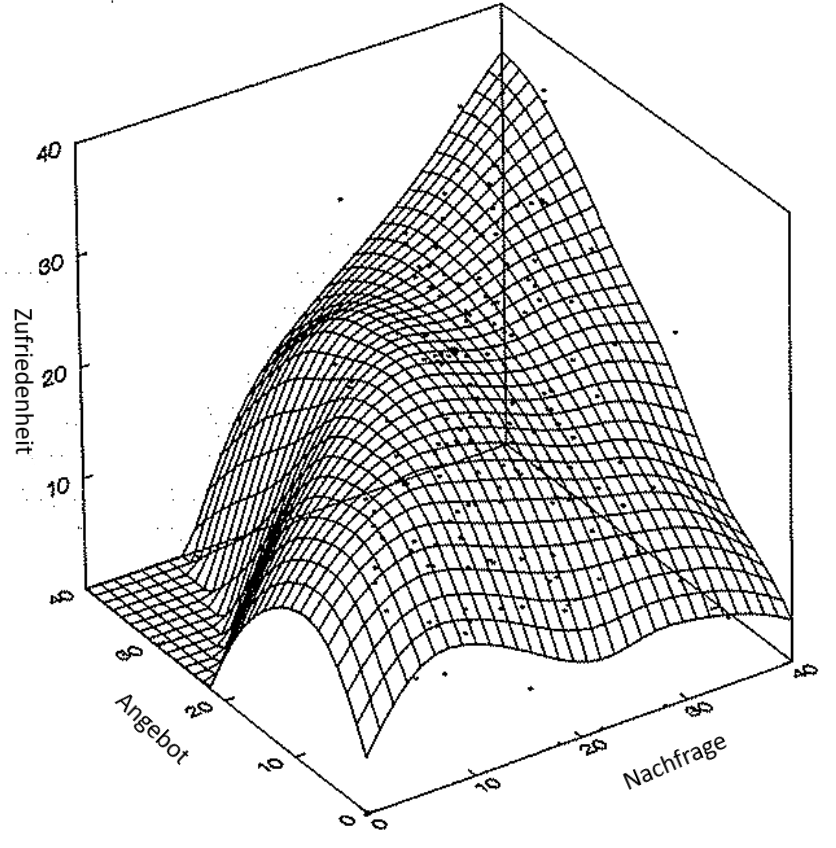
\includegraphics[width=0.6\textwidth]{gfx/drei_d_modell.png}
	\caption{Dreidimensionale Beziehung von P-E Fit und Zufriedenheit \cite[S. 57]{edwards:1991}}
	\label{fig:personEnvironmentFit:wichtigkeiten:abb2}
\end{figure}

Um die stärkere Aussagekraft der Regressionsgleichung zu untermauern, werteten \textcite[S. 18ff.]{edwards:1993b}  in ihrer Publikation einen umfangreichen Datensatz von \textcite[S. 9ff.]{mechanismsOfJobStressAndStrain:1982} erneut aus. Dieser wurde ursprünglich durch Multiplikationen mit Differenzwerten aus Person und Umgebung analysiert. \textcite[S. 18ff.]{edwards:1993b} gelang es, durch Anwendung von Regressionsgleichungen im Vergleich zur erstmaligen Untersuchung einen wesentlich höheren Anteil an Varianz zu erklären \cite[S. 8]{su:2015}.

Um einen solchen Prozess zur Bestimmung des \acp{PEFit} zu Automatisieren, sollten ausreichende Datenmengen der Mitarbeiter zur Berechnung bereitgestellt werden. Beispielsweise beobachteten \textcite[S. 3]{mitre:2014} bei der Analyse von Fähigkeiten in deren erhobenen Daten, dass ein Großteil der Kenntnisse von nur sehr wenigen Mitarbeitern bewertet wurden. In solchen Fällen können Algorithmen eingesetzt werden, welche die unbewerteten Fähigkeiten der Angestellten vorhersagen. Dadurch können die fehlenden Daten ebenfalls in die Berechnung einbezogen werden. Solche Algorithmen kommen unter anderem bei der Implementierung von Empfehlungssystemen zum Einsatz.
%Zu den Analysen von \textcite[S. 18ff.]{edwards:1993b} bzw. \textcite{mechanismsOfJobStressAndStrain:1982} muss betont werden, dass durch die Datenerhebung vorab Kennzahlen zu Person, Umgebung und Ergebnis festgestellt wurden. Die Forscher untersuchten anhand der Daten, über welche Fit-Berechnung am zuverlässigsten auf das Ergebnis geschlossen werden kann.\\
%Neben Edwards stellte auch \textcite[S. 3]{schneider:2001}\cite[S. 2]{schneider:1978} Mängel an bestehenden Person-Environment Fit-Untersuchungen fest. Er betrachtete die Kongruenz von Person und Arbeitsplätzen. Bei der Literaturrecherche bemerkte er, dass bei der Fit-Bestimmung nur selten die vollständige P-E Kongruenz berechnet wird. Meist fokussieren Forscher seinen Beobachtungen zu Folge dabei häufig ausschließlich den Anforderungen-Fähigkeiten Fit. Dieses Phänomen lässt sich auch bei Publikationen zu IT-basierten Empfehlungssystemen dieser Domäne beobachten.
%Um die stärkere Aussagekraft der Regressionsgleichung zu untermauern, werteten \textcite[S. 18ff.]{edwards:1993b}  in ihrer Publikation einen umfangreichen Datensatz von \textcite{mechanismsOfJobStressAndStrain:1982} erneut aus. Dieser wurde ursprünglich durch Multiplikationen mit Differenzwerten aus Person und Umgebung analysiert. \textcite[S. 18ff.]{edwards:1993b} gelang es, durch Anwendung von Regressionsgleichungen im Vergleich zur erstmaligen Untersuchung einen wesentlich höheren Anteil an Varianz zu erklären \cite[S. 8]{su:2015}.
%Zu den Analysen von \textcite[S. 18ff.]{edwards:1993b} bzw. \textcite{mechanismsOfJobStressAndStrain:1982} muss betont werden, dass durch die Datenerhebung vorab Kennzahlen zu Person, Umgebung und Ergebnis festgestellt wurden. Die Forscher untersuchten anhand der Daten, über welche Fit-Berechnung am zuverlässigsten auf das Ergebnis geschlossen werden kann.
%Neben Edwards stellte auch \textcite[S. 3]{schneider:2001}\cite[S. 2]{schneider:1978} Mängel an bestehenden \ac{PEFit}-Untersuchungen fest. Er betrachtete die Kongruenz von Person und Arbeitsplätzen. Bei der Literaturrecherche bemerkte er, dass bei der Fit-Bestimmung nur selten die vollständige P-E Kongruenz berechnet wird. Meist fokussieren Forscher seinen Beobachtungen zu Folge dabei häufig ausschließlich den Anforderungen-Fähigkeiten Fit. Dieses Phänomen lässt sich auch bei Publikationen zu IT-basierten Empfehlungssystemen dieser Domäne beobachten.
\shorthandon{"}